%%%%%%%%%%%%%%%%%%%%%%%%%%%%%%%%%%%%%%%%%
% Programming/Coding Assignment
% LaTeX Template
%
% This template has been downloaded from:
% http://www.latextemplates.com
%
% Original author:
% Ted Pavlic (http://www.tedpavlic.com)
%
% Note:
% The \lipsum[#] commands throughout this template generate dummy text
% to fill the template out. These commands should all be removed when 
% writing assignment content.
%
% This template uses a Perl script as an example snippet of code, most other
% languages are also usable. Configure them in the "CODE INCLUSION 
% CONFIGURATION" section.
%
%%%%%%%%%%%%%%%%%%%%%%%%%%%%%%%%%%%%%%%%%

%----------------------------------------------------------------------------------------
%	PACKAGES AND OTHER DOCUMENT CONFIGURATIONS
%----------------------------------------------------------------------------------------

\documentclass{article}

\usepackage{fancyhdr} % Required for custom headers
\usepackage{lastpage} % Required to determine the last page for the footer
\usepackage{extramarks} % Required for headers and footers
\usepackage[usenames,dvipsnames]{color} % Required for custom colors
\usepackage{graphicx} % Required to insert images
\usepackage{listings} % Required for insertion of code
\usepackage{courier} % Required for the courier font
\usepackage{lipsum} % Used for inserting dummy 'Lorem ipsum' text into the template
\usepackage{hyperref}

% Margins
\topmargin=-0.45in
\evensidemargin=0in
\oddsidemargin=0in
\textwidth=6.5in
\textheight=9.0in
\headsep=0.25in

\linespread{1.1} % Line spacing

% Set up the header and footer
\pagestyle{fancy}
\lhead{} % Top left header
\chead{\hmwkClass: \hmwkTitle} % Top center head
\rhead{\firstxmark} % Top right header
\lfoot{\lastxmark} % Bottom left footer
\cfoot{} % Bottom center footer
\rfoot{Page\ \thepage\ of\ \protect\pageref{LastPage}} % Bottom right footer
\renewcommand\headrulewidth{0.4pt} % Size of the header rule
\renewcommand\footrulewidth{0.4pt} % Size of the footer rule

\setlength\parindent{0pt} % Removes all indentation from paragraphs

%----------------------------------------------------------------------------------------
%	NAME AND CLASS SECTION
%----------------------------------------------------------------------------------------

\newcommand{\hmwkTitle}{Project\ Phase\ 1} % Assignment title
\newcommand{\hmwkDueDate}{Thursday,\ October\ 1,\ 2015} % Due date
\newcommand{\hmwkClass}{Data Modeling and Databases} % Course/class
%\newcommand{\hmwkClassTime}{10:30am} % Class/lecture time
\newcommand{\hmwkClassInstructor}{Qiang Qu} % Teacher/lecturer
\newcommand{\hmwkAuthorName}{Alexey Chernyshov, Vladislav Kravchenko, Murad Magomedov} % Your names

%----------------------------------------------------------------------------------------
%	TITLE PAGE
%----------------------------------------------------------------------------------------

\title{
\vspace{2in}
\textmd{\textbf{\hmwkClass:\ \hmwkTitle}}\\
\normalsize\vspace{0.1in}\small{Due\ on\ \hmwkDueDate}\\
\vspace{0.1in}\large{\textit{\hmwkClassInstructor\ }}
\vspace{3in}
}

\author{\textbf{\hmwkAuthorName}}
\date{} % Insert date here if you want it to appear below your name

%----------------------------------------------------------------------------------------

\begin{document}

\maketitle

%----------------------------------------------------------------------------------------
%	TABLE OF CONTENTS
%----------------------------------------------------------------------------------------

%\setcounter{tocdepth}{1} % Uncomment this line if you don't want subsections listed in the ToC

\newpage
\tableofcontents
\newpage

%----------------------------------------------------------------------------------------
\section{Phase 1. Design and Implement Relational Model.}

\subsection{Introducing}
There are many repositories containing research article information, but not all of them provide interfaces to access this information. Thus we decided to use DBLP. One of its interfaces is (https://aminer.org/billboard/citation), which provides such additional information as cites and abstracts for articles. This information further will be used in ranking methods. 

\subsection{ER-Model}
After studying the documentation we agreed on next entities for our ER-model: 
\begin{itemize} 
	\item Article
	\item Author
	\item Keyword
\end{itemize} 
We will extract Keywords from the abstracts in order to search for related articles.
We designed this ER-Model:
\newline
\begin{figure}[h!]
  \centering
      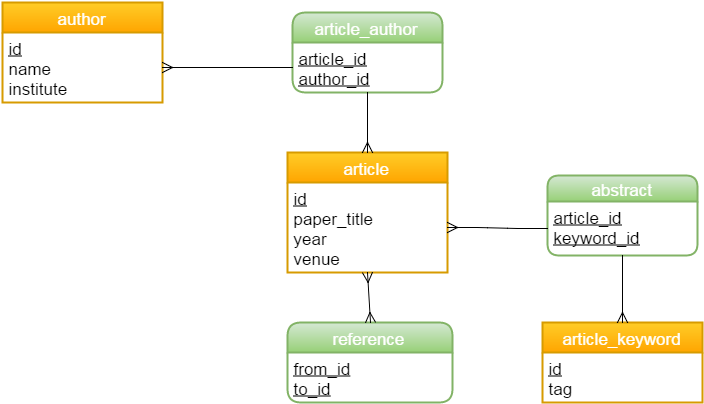
\includegraphics[width=1\textwidth]{ER.png}
  \caption{ER-Model diagram.}
\end{figure}

\newpage
Our ER-Model was transformed into Relations:
\begin{itemize} 
	\item article: \{[\underline{id: INTEGER}, paper\_title: STRING, venue: STRING, year: INTEGER]\}
	\item author: \{[\underline{id: INTEGER}, name: STRING, institute: STRING]\}
	\item keyword: \{[\underline{id: INTEGER}, tag: STRING]\}
	\item article\_author: \{[\underline{id\_article: INTEGER}, \underline{id\_author: INTEGER}]\}
	\item article\_keword: \{[\underline{id\_article: INTEGER}, \underline{id\_keyword: INTEGER}]\}
	\item reference: \{[\underline{from\_id: INTEGER}, \underline{to\_id: INTEGER}]\}
\end{itemize} 

\subsection{Functionality}
We designed the relations in an existing database management system (DBMS) by creating physical tables and their relationships. For our DBMS we have chosen the PostgreSQL. We imported 1.632.442 publications that we parsed using a Python script from an existing publication repository (DBLP).
In addition, we created the SQL-query files that perform such operations:
\begin{itemize} 
	\item Select
	\item Update
	\item Delete
	\item Insert
\end{itemize}
You can search the publication based on author name, publication year, venue(conference/journal name), title, keyword, institution. 

To search for the related articles you can use Keywords and References (to\\from).

You can sort the publications based on such ranking methods:
\begin{itemize} 
	\item based on the number of times the Authors were cited. (In case of a new publication with no references to, but with popular authors)
	\item based on the number of times the Article was cited. (Popular publications)
\end{itemize}
SQL-query files can be found in attachment.


\begin{thebibliography}{1}

\bibitem{def_dblp} 
\url{http://dblp.uni-trier.de/} DBLP

\bibitem{def_aminer} 
\url{https://aminer.org/billboard/citation} aminer.org

\bibitem{def_aminer} 
\url{http://dblp.uni-trier.de/faq/dblpxml[1].pdf} DBLP — Some Lessons Learned by Michael Ley

\bibitem{def_aminer} 
\url{http://dblp.uni-trier.de/xml/docu/dblpxmlreq.pdf} DBLP XML Requests


\end{thebibliography}

\end{document}